\documentclass[a4paper,UTF8]{ctexart}
    \usepackage[T1]{fontenc}
    \usepackage[inner=1in,outer=1.2in,top=1in,bottom=1.2in]{geometry}
    \usepackage{fancyhdr}
    \usepackage{graphicx,subfigure}
    \usepackage{amsfonts,amsmath,listings}
    \usepackage{extarrows}
    \usepackage{enumerate}
    \usepackage{multirow,array,booktabs}
    \usepackage{caption}
    \usepackage{upgreek}
    \usepackage{float}
    \usepackage[colorlinks=true,urlcolor=blue]{hyperref}
    \usepackage[numbers,sort&compress]{natbib}

    
\title{近代物理实验报告}
\author{姓 名\quad 物理学院\quad XXXXXXXXXX}
\date{2020年X月XX日}

% unit
\newcommand{\F}{\mathop{}\negthinspace\mathrm{F}}
\newcommand{\kg}{\mathop{}\negthinspace\mathrm{kg}}
\newcommand{\cm}{\mathop{}\negthinspace\mathrm{cm}}
\newcommand{\um}{\mathop{}\negthinspace\mathrm{\upmu m}}
\newcommand{\mm}{\mathop{}\negthinspace\mathrm{mm}}
\newcommand{\nm}{\mathop{}\negthinspace\mathrm{nm}}
\newcommand{\khz}{\mathop{}\negthinspace\mathrm{kHz}}
\newcommand{\mA}{\mathop{}\negthinspace\mathrm{mA}}
\newcommand{\V}{\mathop{}\negthinspace\mathrm{V}}
\newcommand{\mV}{\mathop{}\negthinspace\mathrm{mV}}
\newcommand{\mw}{\mathop{}\negthinspace\mathrm{mW}}
\newcommand{\uw}{\mathop{}\negthinspace\mathrm{\upmu W}}

\newcommand{\upcite}[1]{\textsuperscript{\textsuperscript{\cite{#1}}}}

\begin{document}
\maketitle

\begin{abstract}
    本次实验观察了A, 测量了B.

    % 此部分为摘要. 200—300字,说明用什么方法做了什么事,由此得到什么结果和结论,有何意义. 摘要中不用缩略词,不用第一人称.
    \paragraph{关键词:} A\quad B

\end{abstract}

\section{引言}
本实验的背景是近代物理实验课程.\upcite{textbook}

% 研究论文引言一般包含以下内容: 
%   所研究领域背景和现状
%   有待研究的问题
%   本研究的目的、主要内容和结果;
%   结果的意义.
% 教学实验肯定不会是原创的. 在写实验报告的引言时,可以假想自己是第一个做类似研究的人.
% 引言一定要切合报告正文,不能漫无目的地介绍背景. 要快速地将读者引导到报告主题上,并作较深入的讨论.
% 引言篇幅可以在较大范围内变化,但最长不应超过报告文字篇幅的1/3.
% 引言撰写可以参考实验讲义,可以复述,但不能复制讲义上的任何一句话.

\section{实验原理}
\subsection{第一小节}
原理一
\subsection{第二小节}
\begin{figure}[H]
    % \setlength{\abovecaptionskip}{0.cm}
    \centering
    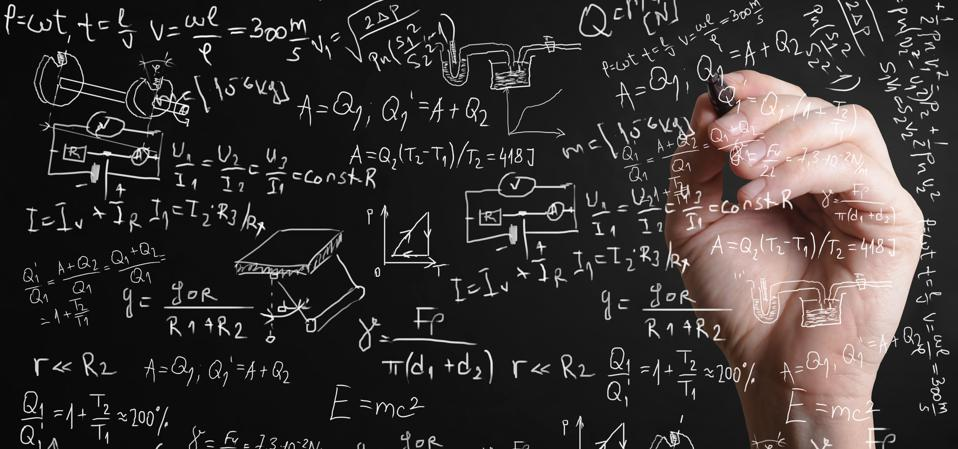
\includegraphics[width=0.9\linewidth]{pic/formula.jpg}
    \caption{实验原理示意图}
    \label{fig:form}
\end{figure}
原理二如图\ref{fig:form}

\section{实验装置与实验方法}
本次实验的装置
% 在此部分需要将实验条件交待清楚到别人能重复你的实验结果的程度. 此外,还需表明你已尽了最大努力来提高实验精度和结果的可靠性. 简单的不确定度估计可以在此节给出,复杂一些的可以放到分析讨论部分.
% 实验条件不仅是指直接影响实验结果的实验参量,而且还包括影响实验质量和可靠性的因素,如室温、空气湿度、基真空、原材料纯度等.
% 作为教学实验报告,此节写详细一点没有坏处.

\section{实验结果与分析}
测量数据和结果

% 此部分是实验报告的主体,应占报告篇幅的一半以上.
% 实验结果应尽量以图表的形式给出. 每一个图表都应该是完整的,即阅读图表时可以不必依赖正文.
% 依自己意愿,实验结果和对结果的分析讨论既可分为两节也可合在一节.
\section{实验结论}
总结
% 首先要给出实验结果,然后再给出由实验结果分析得到的结果和结论.此部分给出的内容要比摘要中的全面,用词要更准确.

\section{致谢}
感谢老师的详细讲解和耐心指导, 感谢同学在实验过程中对我的帮助及与我的讨论.

% 参考文献
\bibliographystyle{unsrt}
\bibliography{ref}

\clearpage
\appendix
\section{思考题}
\paragraph{1. 什么是实验报告?}
\paragraph{2. 怎样写好实验报告?}

% 注: 本次实验报告的全部数据、图片以及代码均已上传至 \href{https://github.com/}{GitHub}

\end{document}
% 本模板参照了孙思白同学发布的报告模板